\documentclass[10pt]{article}
\usepackage{amsmath, amssymb}
\usepackage{amsthm}
\usepackage{graphicx}

\newcommand{\RR}{\mathbb{R}}

\begin{document}

\begin{center}
    \LARGE {Problem Set 2 – Shallow and Deep Networks} \\[1em]
    \Large{DS542 – DL4DS} \\[0.5em]
    \large Spring, 2025
\end{center}

\vspace{2em}

\noindent\textbf{Note:} Refer to the equations in the \textit{Understanding Deep Learning} textbook to solve the following problems.

\vspace{2em}

\section*{Problem 3.2}
For each of the four linear regions in Figure 3.3j, indicate which hidden units are inactive and which are active (i.e., which do and do not clip their inputs).

\begin{figure}[h]
    \centering
    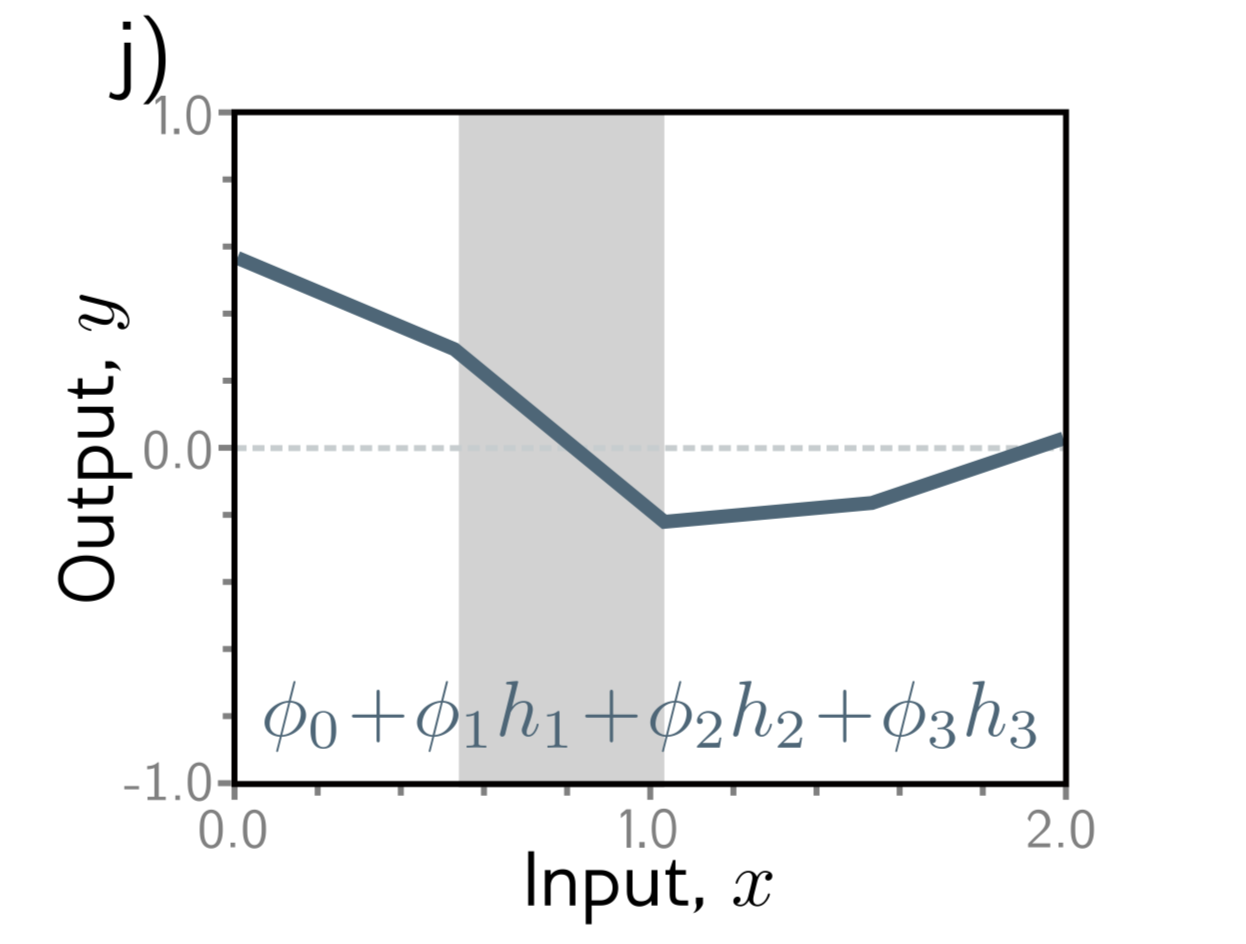
\includegraphics[width=0.5\linewidth]{fig-3.3j.png}
    \caption{Figure 3.3j}
    \label{fig:enter-label}
\end{figure}

\begin{proof}[Solution]
    From the left to the right: 
    
    Region 1: unit 3 is active and units 1, 2 are inactive. 

    Region 2: units 1, 3 are active and unit 2 is inactive. 

    Region 3: all units 1, 2, 3 are active. 

    Region 4: units 1, 2 are active and unit 3 is inactive. 
\end{proof}


\vspace{2em}

\section*{Problem 3.5}

Prove that the following property holds for $\alpha \in \mathbb{R}^+$:
\[
\text{ReLU}[\alpha \cdot z] = \alpha \cdot \text{ReLU}[z].
\]
This is known as the non-negative homogeneity property of the ReLU function.

\begin{proof}
    If \(z \leq 0\), then \(\alpha z \leq 0\). Hence both sides equal to \(0\) as \(\mathrm{ReLU}(x) = 0\) whenever \(x \leq 0\). 

    For \(z>0\), we have \(\alpha z > 0\) since \(\alpha \in \RR^+\). Here \(\mathrm{ReLU}\) behaves the same as identity function, so both sides equal to \(\alpha z\). 
\end{proof}

\vspace{2em}

\section*{Problem 4.6}

Consider a network with $D_i = 1$ input, $D_o = 1$ output, $K = 10$ layers, and $D = 10$ hidden units in each. Would the number of weights increase more -- if we increased the depth by one or the width by one? Provide your reasoning.

\noindent
\textbf{Answer}. The number of weights would increase more if we add the \textbf{width} by $1$. 
\begin{proof}
    The weight matrices have sizes \(\Omega_0 \in \RR^{1 \times 10}, \Omega_{10} \in \RR^{10 \times 1}\), and \(\Omega_k \in \RR^{10 \times 10}\) for \(1 \leq k \leq 9\). Hence there are \(10+10+100 \times 9 = 920\) weights. 

    If we increase depth by $1$, we will add another \(10 \times 10\) weights into the network. In particular, \(\Omega_{10} \in \RR^{10 \times 10}\) and \(\Omega_{11} \in \RR^{10 \times 1}\). There will be \(10+10+100 \times 10 = 1020\) weights in total. 

    If we increase width by $1$, then \(\Omega_k \in \RR^{11 \times 11}\) for \(1 \leq k \leq 9\). Thus we are adding \(21\) weights to each layers. Moreover, \(\Omega_0, \Omega_{10}\) would also increase their size by \(1\). The total number of weights increased is \(21 \times 9 + 2 = 191\), which is more than increasing depth by \(1\). 
\end{proof}


\end{document}
